
\section{Background}
\label{sec:theory_presentations}
In order to handle theory presentations and manipulate them, we need to arrive at a concrete 
definition of what they are. This section sets the ground for our work. We define theory 
presentations from our perspective in Section \ref{sec:ThryPres}. The library that we will use in this 
work comes from MathScheme system. It is introduced in Section \ref{sec:MathScheme}. As a 
preprocessing step to working on the library, we translate it to MMT, another formalization system 
that we introduce in Section \ref{sec:MMT}. We benefit from the translation by expanding the team 
working on the library and having access to more resources, like web interface, graph viewer and a 
latex processor.

\subsection{Theory Presentations}
\label{sec:ThryPres}
According to \cite{farmer2007biform}, a general language $L$ can be defined as a pair $(\mathcal{E} , 
\mathcal{F})$ such that $\mathcal{E}$ is a set of syntactic entities and $\mathcal{F} \subseteq 
\mathcal{E}$ is a set of formulas in $L$. A general logic is a set of general languages with some notion 
of logical consequence. A theory in  some language $L$ is the declaration of the syntactic entities and 
a set of formulas closed under the notion of logical consequence provided by the underlying logic. 
The focus of our work is to mechanize the generation of algebraic structures from theory presentations. Therefore, we need to focus on a syntactic representation that corresponds to the concept of a theory. 
A theory presentation for us is a specification from which a theory could be generated. Instead of 
containing all possible formulas, as in a theory, a theory presentation contain only the kernel from 
which all formulas could be generated. Since we are interested in typed languages, we consider theory 
presentations that allow definitions of new types, declarations of typed symbols, definitions of these 
symbols (in the form of lambda expressions) and axioms describing them. The semantics of a theory 
presentation is the corresponding abstract theory in logic. 

A theory presentation gives the means of writing down a theory in a formal language. It provides 
means to define the components of the kernel of a theory. Our notion of theory presentations is not 
only limited to proof assistants. Different systems incorporate some form of theory presentation under 
different names; for example module signatures (as in Ocaml), data definitions (as in Agda), class 
definitions (as in Coq, Isabelle and Lean), record definitions (as in Agda and Coq), type classes (as in 
Haskell), traits (as in Scala) and others holding similar structures of having types, constants, 
functions, predicates and lambda expressions. In \cite{MFK2018TheoriesAsTypes}, a correspondence is 
established between the following concepts from theorem provers and programming languages: 
theories, record types, modules, ML signatures, C++ and java classes. We understand that they have 
different features. Part of this work is to explore their commonalities and differences. 

We use MathScheme library to run our experiments. The MathScheme system is introduced in the next 
section. 


\subsection{MathScheme}
\label{sec:MathScheme}
MathScheme \cite{Carette2011} is a mechanized mathematics system being developed at McMaster University. It offers a library of over 1000 theory presentations \cite{carette2011mathscheme, zhang2009language} defined in the MathScheme language. The theories are defined by means of theory combinators \cite{carette2012theory}. Three main combinators are used 
\begin{itemize}
	\item Extends: A theory $B$ is an extension of a theory $A$ if all declarations of $A$ are contained in $B$, but not all declarations of $B$ are contained in $A$. 
	\item Renames: A theory $B$ is a rename of theory $A$ if it renames one or more of the declarations in $A$. 
	\item Combines: A theory $C$ combines two theories $A$ and $B$ by computing the pushout of the 
	two theory presentations in the category of theories and theory morphisms. The resulting theory 
	includes all the declarations of the two theories, gluing together those that can be traced back to 
	the source. 
\end{itemize} 
Defining theories using those combinators result in a theory graph in which theories are the nodes 
and theory morphisms are the edges. MathScheme also employs the little 
theories approach \cite{farmer1992little} in which theories are defined incrementally by adding 
minimal details at each increment. This way allows theorems to be proved using minimal 
axiomatizations which provides maximum generality. 
The system implements a flattener that outputs the expanded theory presentation as would be seen in a mathematics textbook. In this work, we consider theories in their flattened format. This gives us access to its components, which we need in order to manipulate the theories. As part of the collaboration between MathScheme and MMT projects, the library is being translated into MMT language to provide more support and expand the development team. 


\subsection{MMT}
\label{sec:MMT}
MMT \cite{MMT_homepage}
is a framework for representing mathematical knowledge. It is based on two design concepts; foundation independence and modularity. 

Foundation independence avoids the commitment to any specific logical framework and allows the translation between them. This way, it enables interoperability and reuse. MMT realizes foundation independence by representing core mathematical knowledge as theories (logics-as-theories approach). 

Modularity is realized by linking the theories via theory-morphisms \cite{rabe2008exchange}. 
MMT defines three types of theory morphisms; inclusions, structures and views\cite{mathhubTut2017}. Morphisms created via inclusion make the declarations of one theory included in the other without any change in the source theory. Structures are named inclusions that allow changing notations or definitions of symbols of the source theory. Views map symbols of the source theory to those of the target one.
Meta-theory relation is one form of theory morphisms. Meta-theories are useful to achieve both 
modularity and foundation independence. They act as the language infrastructure for their 
descendants to be able to present domain-specific knowledge. We write $M/T$ to denote that theory 
$T$ is defined using the meta-theory $M$. This implies that the semantics of $T$ can only be given 
with respect to the semantics of $M$.

Using logics-as-theories and theory morphism approaches induce a theory graph structure on the MMT library, where nodes are theories and arcs are theory morphism relations. Figure \ref{MMT_Library_LF} shows part of the theory graph in the MMT library. The graph shows that the $\mathsf{LF/FOL/Monoid}$, $\mathsf{LF/FOL/cgroup}$ and $\mathsf{LF/FOL/Ring}$ theories all have the same foundation (meta-theory) . They are defined in $\mathsf{FOL}$, but can be translated to $\mathsf{HOL}$ via the $m^\prime$ morphism. 
\begin{figure}
	\centering
	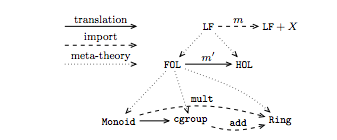
\includegraphics[scale = 1.0]{figures/MMT_Library_LF.png}
	\caption{Part of the MMT theory graph \cite{kohlhase2016qed}.}
	\label{MMT_Library_LF}
\end{figure} 

\begin{comment}
The grammar defining a flattened theory in MMT is defined in Figure 

\begin{figure}
\begin{lstlisting}
$\Gamma$ ::= $\cdot$ | $\Gamma$ , x [:$T$] [:=$T$]
$T$ ::= x | type | kind | $\Pi_{x : T^\prime} T$ | $\lambda x : T^{\prime} . T$ | $T_1T_2$
$\Theta$ ::= $\cdot$ | $\Theta, X = \{\Gamma\}$ | $\Theta, X : X_1 \rightarrow X_2 = \{\Gamma\}$
\end{lstlisting}
\label{fig:thy_pres_mmt}
\caption{The grammar for flattened theories in MMT. $\Gamma$ is a}
\end{figure}
\end{comment}

MathScheme and MMT share many of the main ideas of representing theories. This is one reason why merging both systems is being done. 